\documentclass{oxmathproblems}
\usepackage{graphicx}
\usepackage{hyperref}
\usepackage{footmisc}
\usepackage{listings}
\usepackage{color}
\usepackage{xcolor}
\graphicspath{{imagenes/}} 

\course{EE447 Mobile Internet HW 4\\ Heterogeneous Graphs}

\newtheorem{theorem}{Theorem}
\newtheorem{lemma}[theorem]{Lemma}
\newtheorem{proposition}[theorem]{Proposition}
\newtheorem{corollary}[theorem]{Corollary}
\newtheorem{exercise}{Exercise}
\newtheorem{definition}{Definition}
\theoremstyle{definition}
\lstset{
	keywordstyle=\color{blue!70}\bfseries, %设置关键词为蓝色,需要引xcolor宏包
	basicstyle=\ttfamily\footnotesize, 
	commentstyle=\ttfamily, %基本和注释的字体都使用默认的等宽,而非texlive调用的中文字体
	showstringspaces=false, %不显示中间的空格
	frame=shadowbox,
	rulesepcolor=\color{red!20!green!20!blue!20},
}
\makeatletter \renewenvironment{proof}[1][Proof] {\par\pushQED{\qed}\normalfont\topsep6\p@\@plus6\p@\relax\trivlist\item[\hskip\labelsep\bfseries#1\@addpunct{.}]\ignorespaces}{\popQED\endtrivlist\@endpefalse} \makeatother
\makeatletter
\renewenvironment{solution}[1][Solution] {\par\pushQED{\qed}\normalfont\topsep6\p@\@plus6\p@\relax\trivlist\item[\hskip\labelsep\bfseries#1\@addpunct{.}]\ignorespaces}{\popQED\endtrivlist\@endpefalse} \makeatother

\begin{document}
\begin{center}
	% Please write down your name, student id and email.
	Name: Hongjie Fang \quad Student ID:518030910150 \quad Email: \href{mailto:galaxies@sjtu.edu.cn}{galaxies@sjtu.edu.cn}
\end{center}
\textbf{Problem}\footnote{Translated by DeepL Translator: \url{https://www.deepl.com/translator}}.

Given 5 identical nodes, how many different networks can be built? Use symmetry and complementarity to enumerate as few network structures as possible.

Symmetry: As shown in the figure below, two diagrams remain isomorphic under different edge relations, and only one of them should be included in the enumeration of ``networks that are not isomorphic to each other''.
\begin{figure}[htbp]
	\centering
	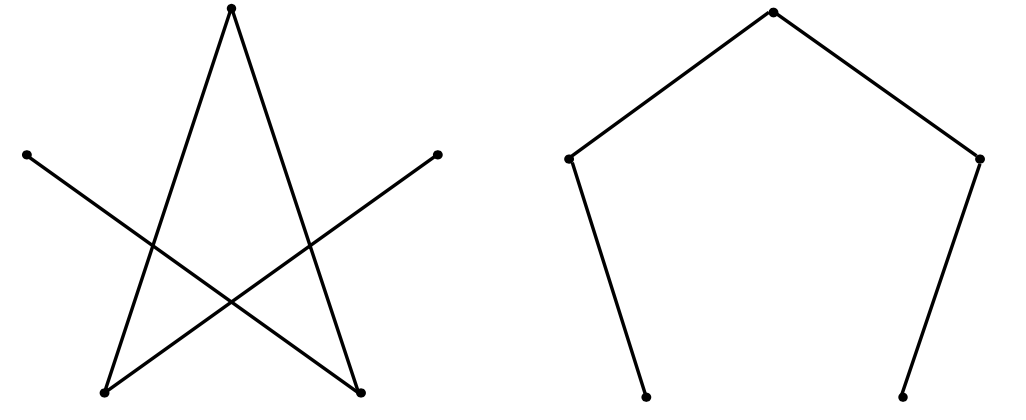
\includegraphics[width=0.5\linewidth]{1.png}
	\label{fig1}
\end{figure}

Complementarity: As shown in the figure below, the two diagrams overlap to form a complete diagram, so the former structure can be directly derived from the latter structure given in the enumeration.
\begin{figure}[htbp]
	\centering
	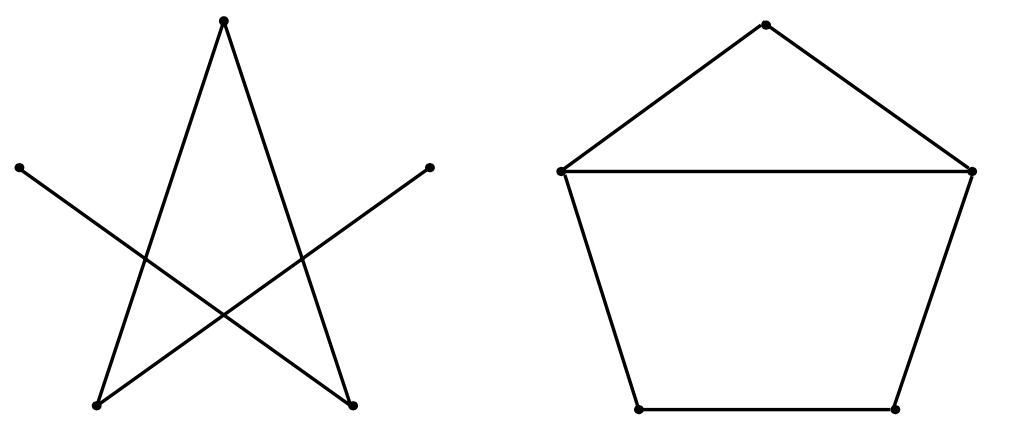
\includegraphics[width=0.5\linewidth]{2.png}
	\label{fig2}
\end{figure}
\begin{solution}
	First we consider complementarity. Since there is totally $5\times (5 - 1) \times \frac{1}{2} = 10$ edges in a graph which consists of $5$ identical nodes, we just need to enumerate the number of edges from $0$ to $5$ to eliminate complementarity, which is based on the following lemmas.

	\begin{lemma}\label{lemma1} For a graph consists of $n$ nodes and $m$ edges, there is a corresponding graph consists of $n$ nodes and $\left(\frac{n(n-1)}{2} - m\right)$ edges as its complementary graph; and vice versa.
	\end{lemma}
	\begin{lemma}\label{lemma2} For two heterogeneous graphs which consists of $n$ nodes and $m$ edges each, their complementary graphs are also heterogeneous; and vice versa.
	\end{lemma}

	From Lemma \ref{lemma1} and Lemma \ref{lemma2} we can draw the conclusion that we can enumerate $m$ from $0$ to $\left\lceil\frac{n(n-1)}{4}\right\rceil$ to count the heterogeneous graphs.

	Then, let us consider that the number of heterogeneous graphs which consist of $n$ nodes and $m$ edges, where $0 \leq m \leq \left\lceil\frac{n(n-1)}{4}\right\rceil$. In the settings of this problem, we just need to count the number of heterogeneous graphs of $n = 5$ and $0 \leq m \leq 5$. For graphs of $n$ nodes and $m$ edges, we can enumerate the degree of nodes to prevent omissions. For example, when $n = 5$ and $m = 4$, the sum of node degrees will be $2m = 8$, therefore we can enumerate the multi-set of node degrees such as $[4, 1, 1, 1, 1]$, $[3, 2, 2, 1, 0]$, $[3, 2, 1, 1, 1]$, $[2, 2, 2, 1, 1]$ and $[2, 2, 2, 2, 0]$, and the corresponding graphs are listed as Fig. \ref{fig3} shown.

	\begin{figure}[htbp]
		\centering
		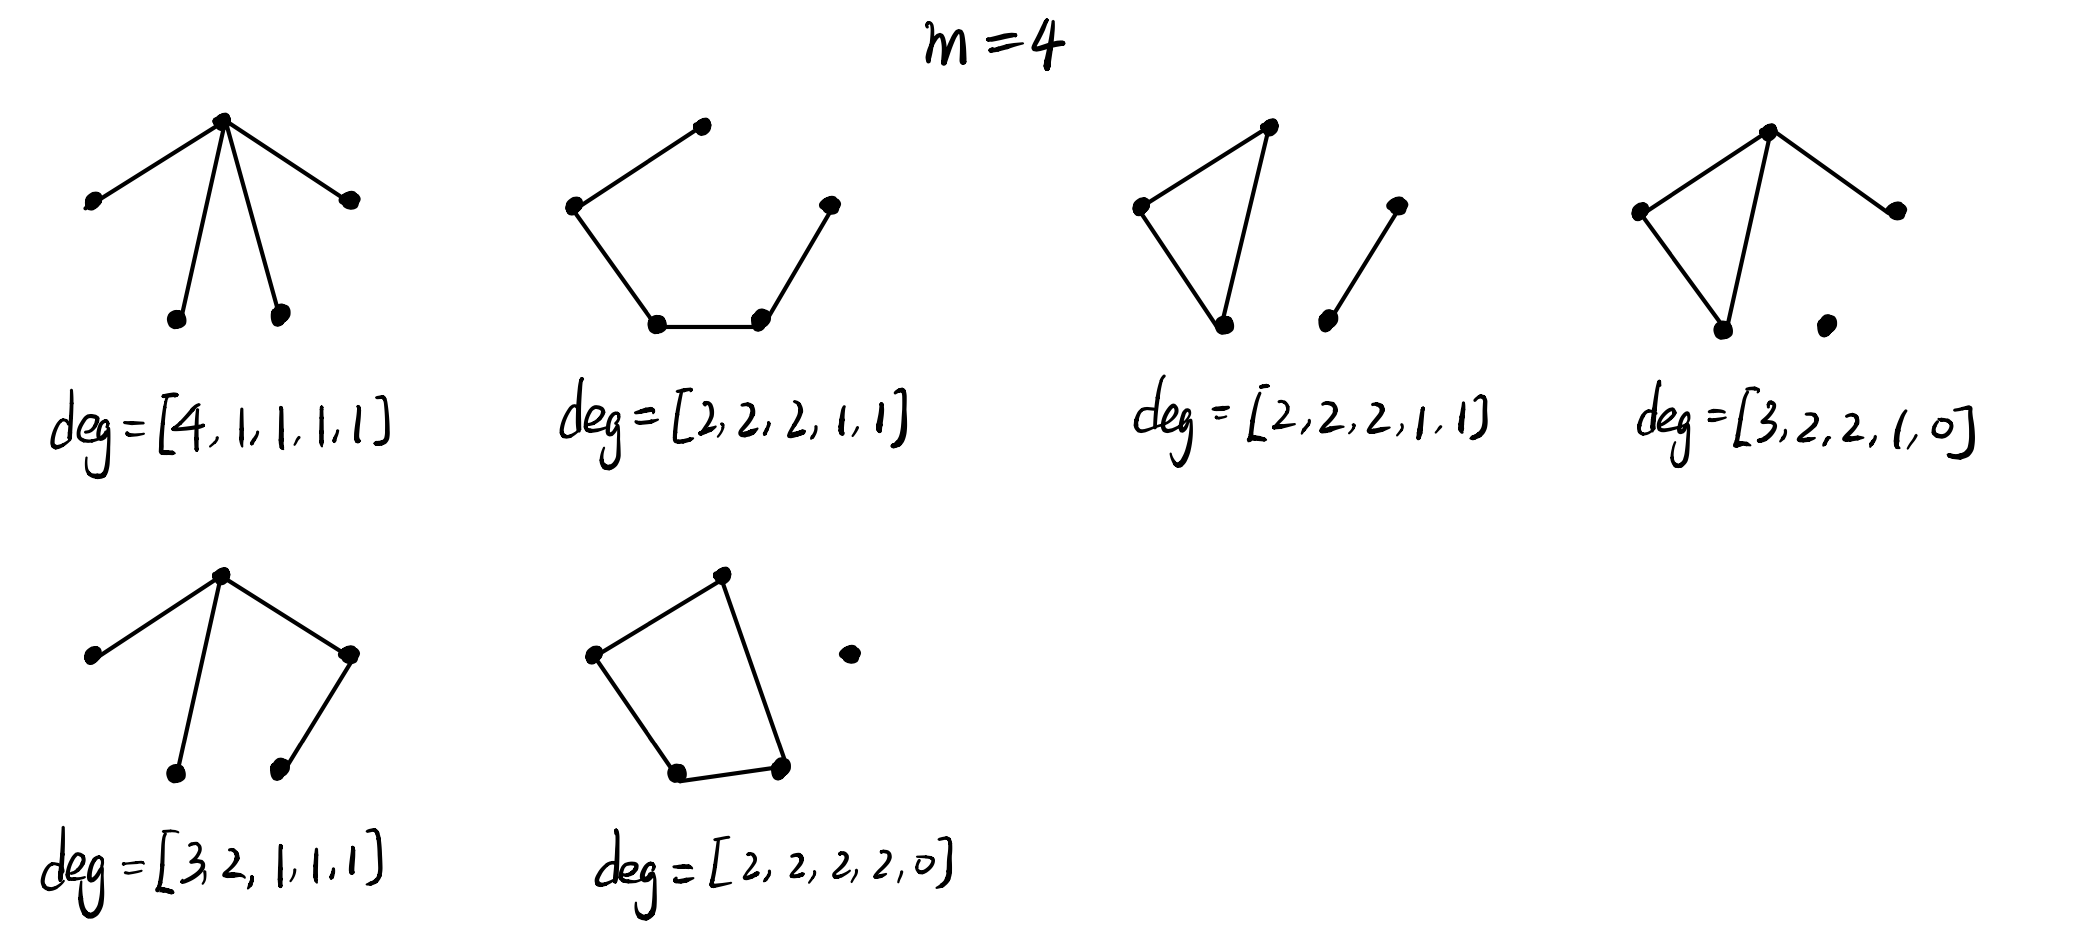
\includegraphics[width=0.8\linewidth]{3.png}
		\caption{The heterogeneous graphs when $n = 5, m = 4$.}
		\label{fig3}
	\end{figure}

	Similarly, we can list the heterogeneous graphs when $m = 0, 1, 2, 3$ and $m = 5$, as shown in Fig. \ref{fig4} and Fig. \ref{fig5}.

	\begin{figure}[htbp]
		\centering
		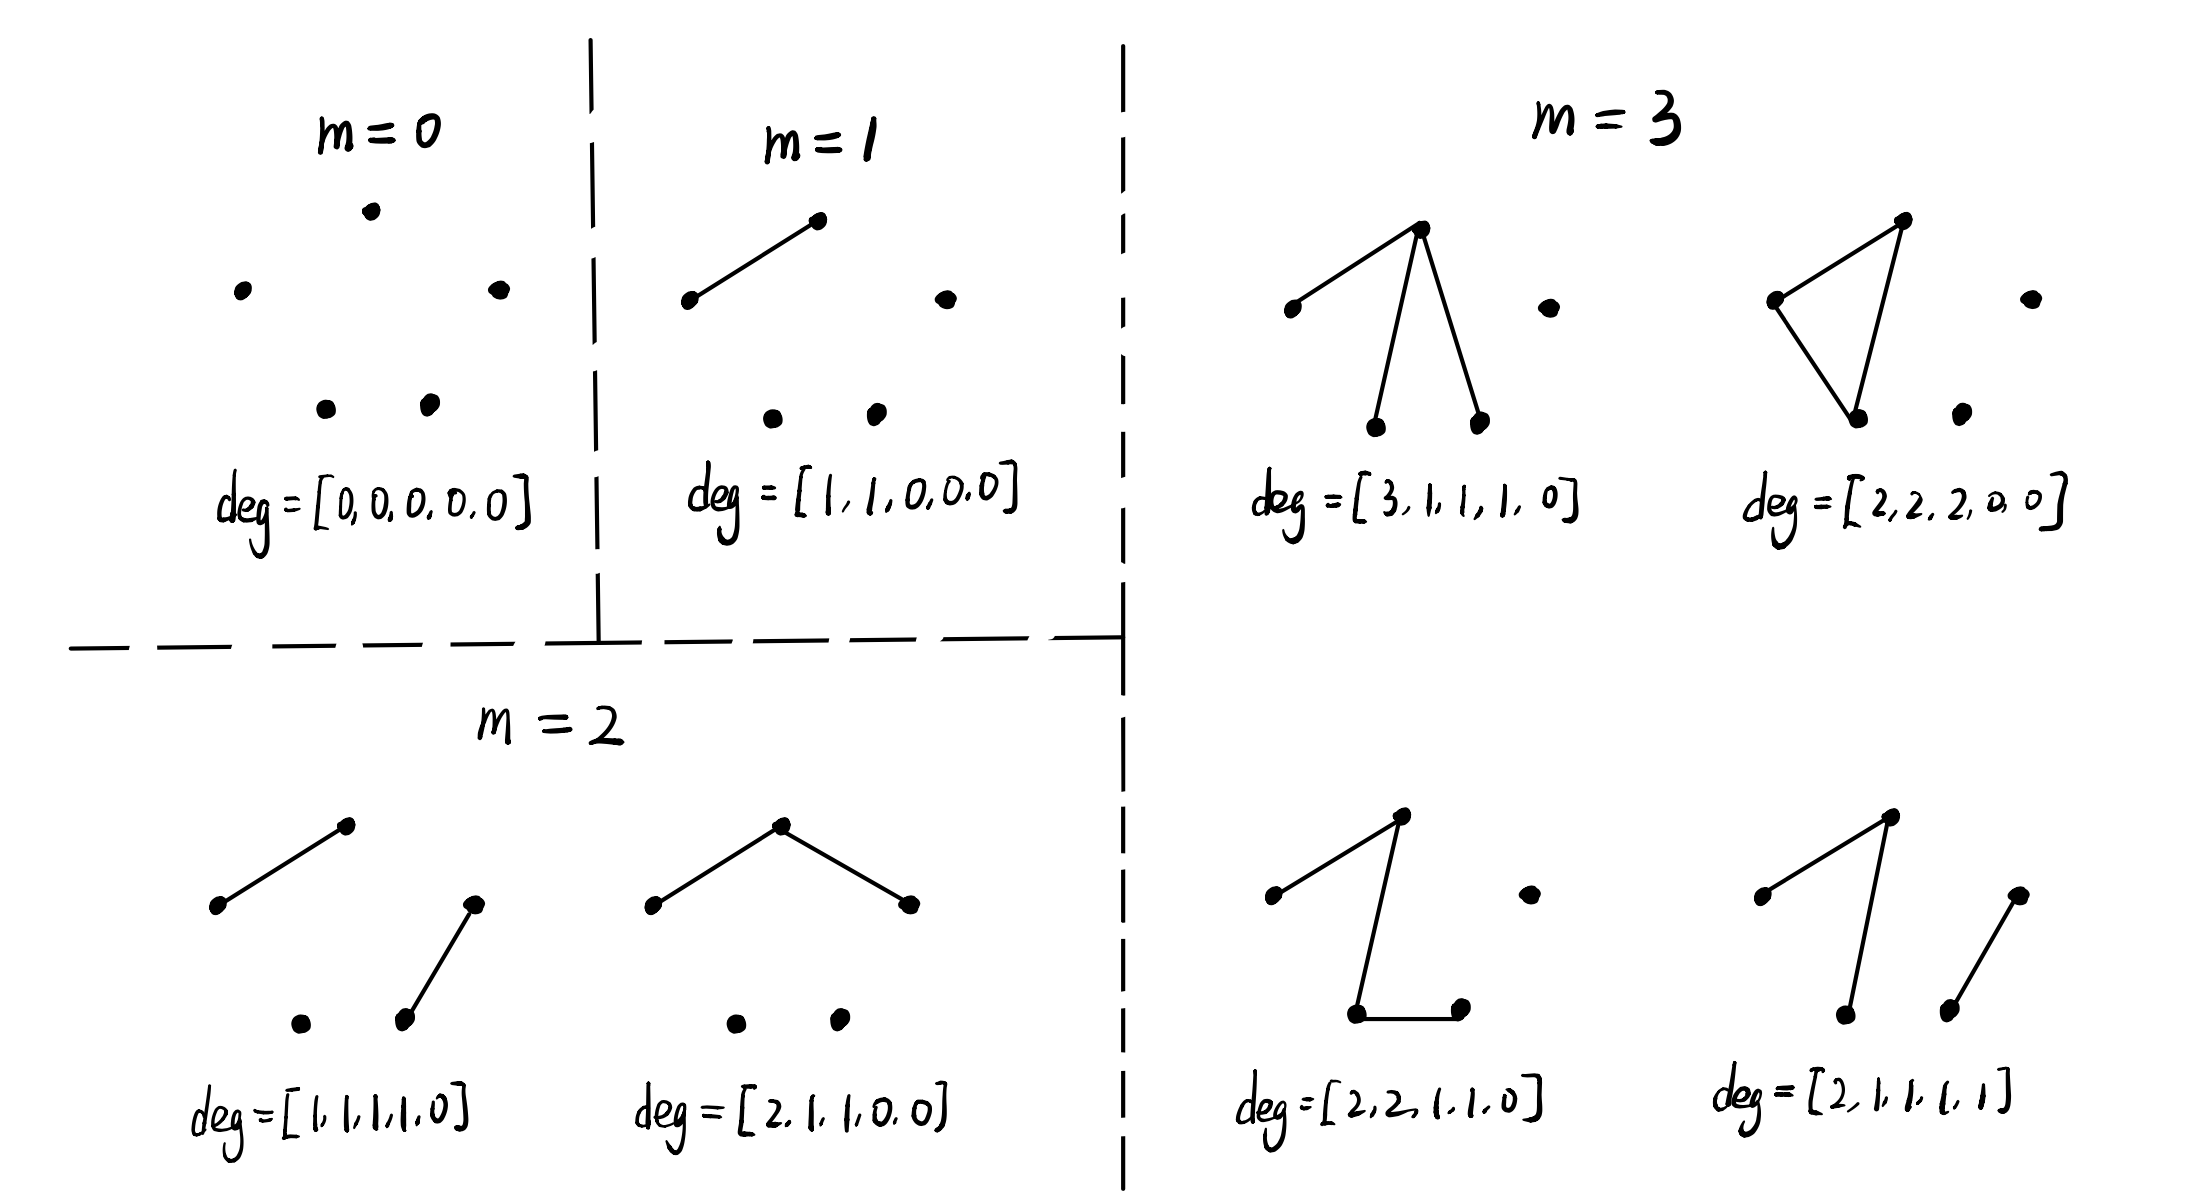
\includegraphics[width=0.8\linewidth]{4.png}
		\caption{The heterogeneous graphs when $n = 5, m = 0, 1, 2, 3$.}
		\label{fig4}
	\end{figure}

	\begin{figure}[htbp]
		\centering
		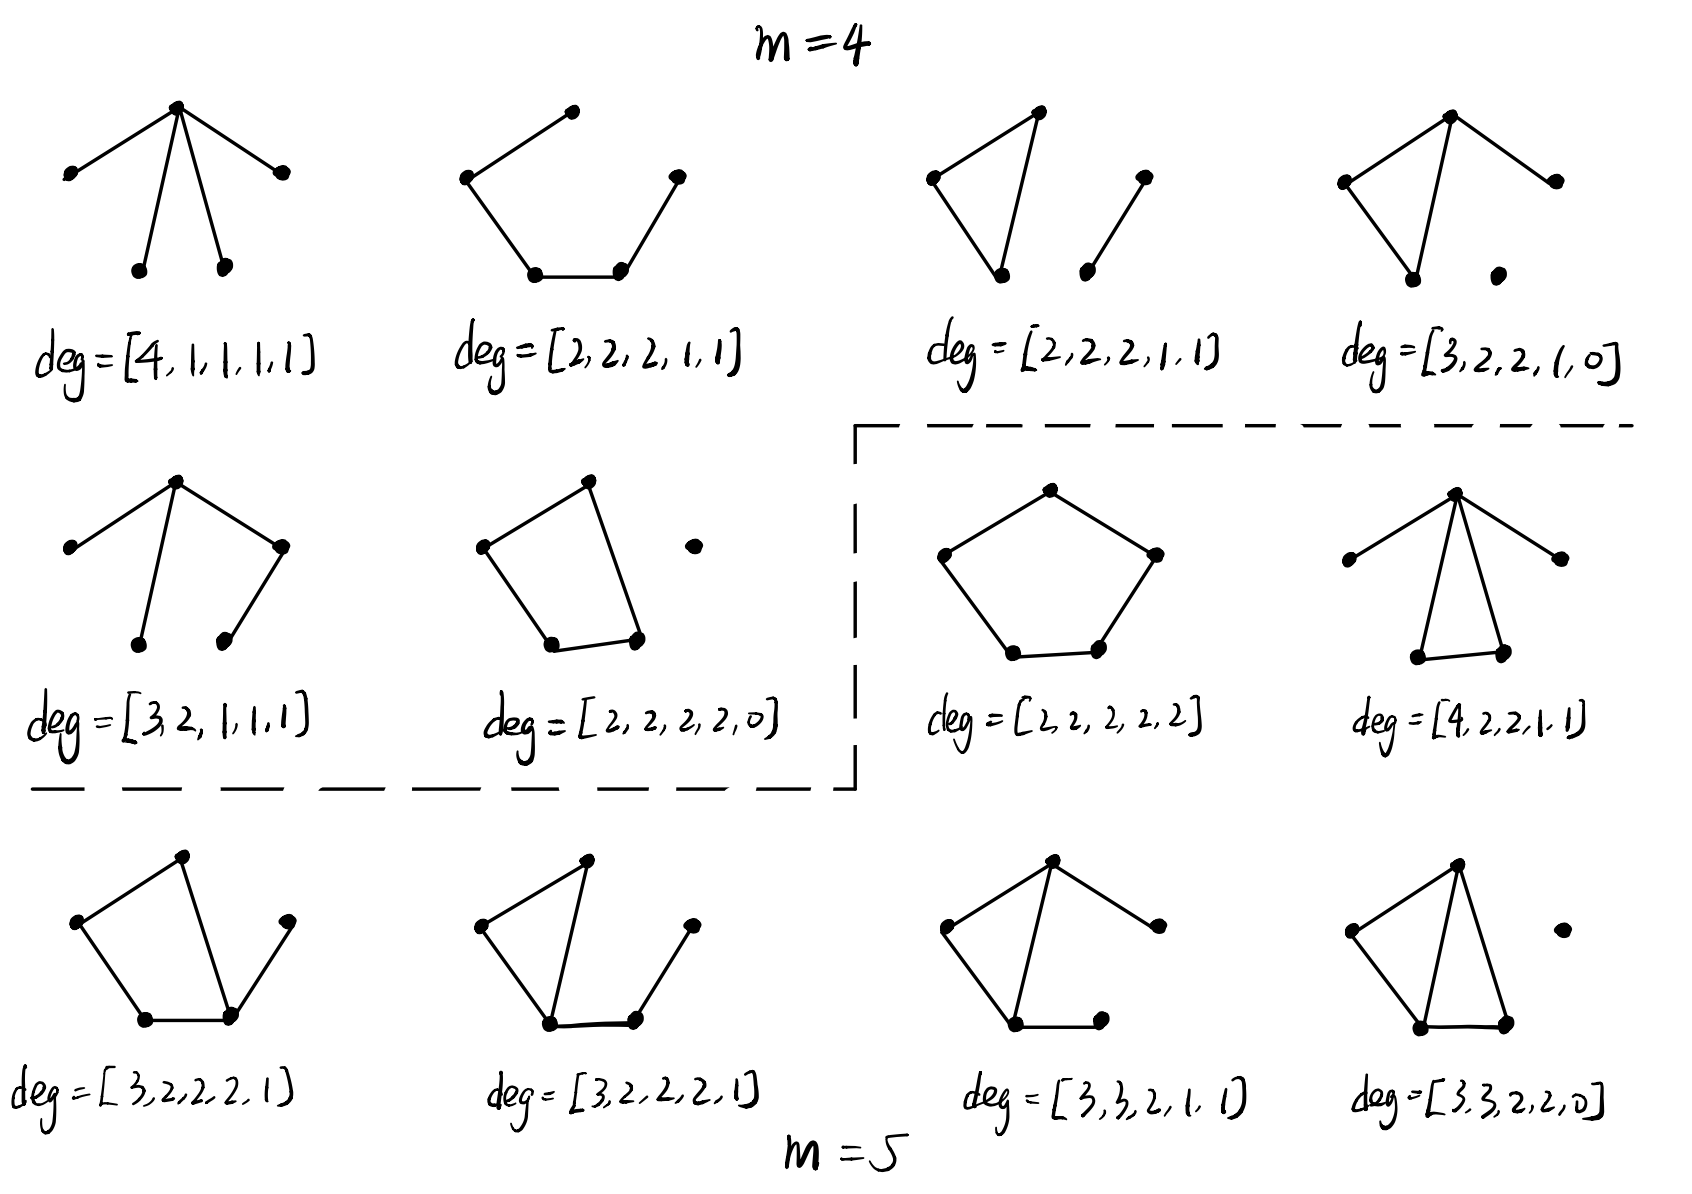
\includegraphics[width=0.8\linewidth]{5.png}
		\caption{The heterogeneous graphs when $n = 5, m = 4, 5$.}
		\label{fig5}
	\end{figure}

	Notice that for $m = 5$, since $2m = 10 = \frac{n(n-1)}{2}$, the complementarity are inside the graph set of $m = 5$. Suppose for $n$ nodes and $m$ edges, there are $N(n,m)$ heterogeneous graphs. Therefore Lemma \ref{lemma1} and Lemma \ref{lemma2} states that,

	$$
	N(n,m) = N\left(n,\frac{n(n-1)}{2} - m\right)
	$$

	Combining the previous lemmas with the result in Fig. \ref{fig4} and Fig. \ref{fig5}, we can know that 

	\begin{itemize}
		\item $N(5, 0) = 1$;
		\item $N(5, 1) = 1$;
		\item $N(5, 2) = 2$;
		\item $N(5, 3) = 4$;
		\item $N(5, 4) = 6$;
		\item $N(5, 5) = 6$;
		\item $N(5, 6) = N(5, 4) = 6$;
		\item $N(5, 7) = N(5, 3) = 4$;
		\item $N(5, 8) = N(5, 2) = 2$;
		\item $N(5, 9) = N(5, 1) = 1$;
		\item $N(5, 10) = N(5, 0) = 1$;
	\end{itemize}

	Therefore, for $n = 5$, there are totally

	$$
	\sum_{m=0}^{\frac{5\cdot(5-1)}{2}} N(5, m) = 34
	$$
heterogeneous graphs, that is, given $5$ identical nodes, totally $34$ different networks can be built. We can double-check the result using OEIS\footnote{\url{http://oeis.org/}}, an online encyclopedia of integer sequences website. As shown in Fig. \ref{fig6}, we can see that our result is correct.

\begin{figure}[htbp]
	\centering
	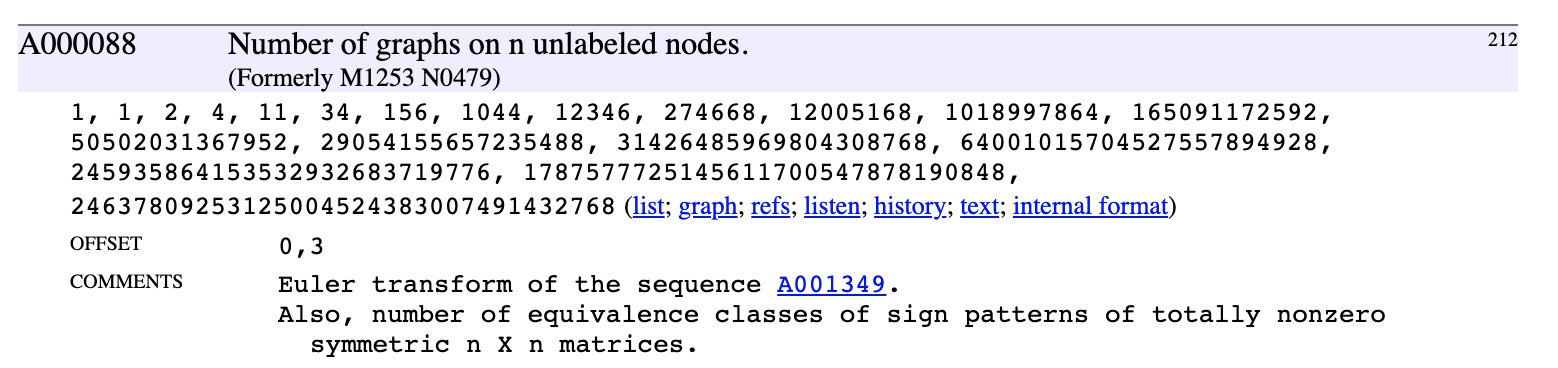
\includegraphics[width=\linewidth]{6.png}
	\caption{The result using OEIS}
	\label{fig6}
\end{figure}


\end{solution}
\end{document}
